
\chapter{Observation modes}

\begin{table}
\caption{ \smr\ operational modes in aeronomy  for AC1 and AC2
and the sub-mm frontends (FM = frequency mode)}
\label{table:config2}
\begin{tabular}{|l|l|l|l|l|}
  \hline
  \textbf{Backend} & \textbf{Frontend} & \textbf{LO freq {[}GHz{]}} & \textbf{Source mode} & \textbf{FM} \\
  \hline
   AC1             & 495 A2            &  492.750                   & Transport            & 23 \\
  \cline{3-3}
  \cline{4-4}
  \cline{5-5}
                  &                    & 499.698                    & Transport            & 25 \\
  \cline{2-2}
  \cline{3-3}
  \cline{4-4}
  \cline{5-5}
                  & 549 A1            & 548.502                    & Stratospheric         & 2 \\
  \cline{3-3}
  \cline{4-4}
  \cline{5-5}
                  &                   & 553.050                    & Water isotope         & 19 \\
  \cline{3-3}
  \cline{4-4}
  \cline{5-5}
                  &                   & 547.752                    & Water isotope         & 21 \\
  \cline{3-3}
  \cline{4-4}
  \cline{5-5}
                  &                   & 553.302                    & Transport             & 23 \\
  \cline{2-2}
  \cline{3-3}
  \cline{4-4}
  \cline{5-5}
                 & 555 B2             & 553.298                    & Summer mesosphere     & 13 \\
  \cline{2-2}
  \cline{3-3}
  \cline{4-4}
  \cline{5-5}
                & 572 B1             & 572.762                     & Transport             & 24 \\
  \hline
  AC2           & 495 A2             & 497.880                     & Stratospheric         & 1 \\
  \cline{3-3}
  \cline{4-4}
  \cline{5-5}
                &                    & 492.750                     & Water isoptope        & 8 \\
  \cline{3-3}
  \cline{4-4}
  \cline{5-5}
                &                    & 494.750                     & Water isotope         & 17 \\
  \cline{3-3}
  \cline{4-4}
  \cline{5-5}
                &                    & 499.698                     & Transport             & 25 \\
  \cline{2-2}
  \cline{3-3}
  \cline{4-4}
  \cline{5-5}
                & 572 B1             & 572.762                     & Summer mesosphere     & 14 \\
  \cline{3-3}
  \cline{4-4}
  \cline{5-5}
                &                    & 572.964                     & Transport            & 22 \\
\hline
\end{tabular}
\end{table}

\begin{table}
\caption{ \smr\ frontend and backend frequency specification for modes that are measured 
during part of the summer (when only backend AC2 is used, which is the case for 2013 and onwards). 
These modes are normally measured by backend AC1 (e.g. FM 102 and FM 2, FM 119 and FM 19, 
FM 121 and FM 21, and FM 113 and 13, are all identical except the Backend used).}
\label{table:config3}
\begin{tabular}{|l|l|l|l|l|}
  \hline
  \textbf{Backend} & \textbf{Frontend} & \textbf{LO freq {[}GHz{]}} & \textbf{Source mode} & \textbf{FM} \\
  \hline
  AC2              & 549 A1            & 548.502                    & Stratospheric        &  102 \\
  \cline{3-3}
  \cline{4-4}
  \cline{5-5}
                   &                   & 553.050                    & Water isotope        & 119 \\
  \cline{3-3}
  \cline{4-4}
  \cline{5-5}
                   &                   & 547.752                    & Water isotope        & 121 \\
  \cline{2-2}
  \cline{3-3}
  \cline{4-4}
  \cline{5-5}
                   & 555 B2            & 553.298                    & Summer mesosphere    & 113 \\
  \hline
\end{tabular}
\end{table}




\begin{table}
\caption{ \smr\ frontend and backend frequency specification}
\label{table:config4}
\begin{tabular}{|l|l|l|l|l|l|}
  \hline
  \textbf{FM} & \textbf{SMR mode} & \textbf{LO Freq.} & \textbf{Freq. Range} & \textbf{Species}                    & \textbf{Name / ID} \\
              &                   & {[}GHz{]}         & {[}GHz{]}            &                                     &                    \\
  \hline
  01          & s1a or sc1a       & 497.880           & 501.180--501.580    & \chem{ClO}, \chem{O_3}, \chem{N_2O} & SM-AC2a / 01 \\
  \cline{2-2}
  \cline{3-3}
  \cline{4-4}
  \cline{6-6}
              &                   &                   & 501.980--502.380    &                                     & SM-AC2b / 02 \\
  \cline{2-2}
  \cline{3-3}
  \cline{4-4}
  \cline{6-6}
             &                    &                   &                      &                                                    & SM-AC2ab / 29 \\
  \hline
  02         & s1a                & 548.502           & 544.102--544.902    & \chem{HNO_3} , \chem{O_3}                          & SM-AC1e / 03 \\
  \hline
  08         & w3a or w5a         & 492.750           & 488.950--489.350    & \chem{H_{2}^{18}O}, \chem{O_3},\chem{H_{2}^{16}O}  & IM-AC2a / 13 \\
  \cline{2-2}
  \cline{3-3}
  \cline{4-4}
  \cline{6-6}
             &                    &                   & 488.350--488.750    &                                                    & IM-AC2b / 14 \\
  \cline{2-2}
  \cline{3-3}
  \cline{4-4}
  \cline{6-6}
            &                     &                   &                      &                                            & IM-AC2ab / 30 \\
  \hline
  17        & w4a or w5b          & 494.250           & 489.950--490.750    & \chem{HDO}, \chem{{18}^O_3}                & IM-AC2c / 21 \\
  \hline
  19        & w3a or w4a          & 553.050           & 556.550--557.350    & \chem{H_2O}, \chem{O_3}                    & IM-AC1c / 22 \\
  \hline
  21        & w5a or w5b          & 547.752           & 551.152--551.552    & \chem{NO}, \chem{O_3}, \chem{H_{2}^{17}O}  & IM-AC1de / 31 \\
  \cline{2-2}
  \cline{3-3}
  \cline{4-4}
  \cline{6-6}
            &                     &                   & 551.752--552.152    &                                                       &  \\
  \hline
  13        & sm1a                & 553.298           & 556.598--557.398    & \chem{H_{2}^{16}O}, \chem{O_3}                        & HM-AC1c / 19 \\
  \hline
  14        & sm1a                & 572.762           & 576.062--576.862    & \chem{CO}, \chem{O_3}                                 & HM-AC2c /20 \\
  \hline
  22        & co1a                & 572.964           & 576.254--576.654    & \chem{CO}, \chem{O_3}, \chem{HO_2},\chem{^{18}O_3}    & HM-AC2ab / 32 \\
  \cline{2-2}
  \cline{3-3}
  \cline{4-4}
  \cline{6-6}
            &                     &                   & 577.069--577.469    &                                      &  \\
  \hline
  23        & co1a                & 492.750           & 488.350--488.750    & \chem{H_{2}^{16}0}, \chem{O_3}       & HM-AC1d / 33 \\
  \cline{2-2}
  \cline{3-3}
  \cline{4-4}
  \cline{6-6}
            &                     & 553.302           & 556.702--557.102    &                                      & HM-AC1e / 34 \\
  \hline
  24        & sc1a                & 572.762           & 576.062--576.862    & \chem{CO}, \chem{O_3}                & HM-AC1e / 35 \\
  \hline
  25        & ut1a                & 499.698           & 502.998--504.198    & \chem{H_{2}^{16}O}, \chem{O_3}       & TM-ACs1 / 36 \\
\hline
\end{tabular}
\end{table}


%\chapter{Coverage in time}

\chapter{Time series of Level0 and Level1B data}

\begin{figure}
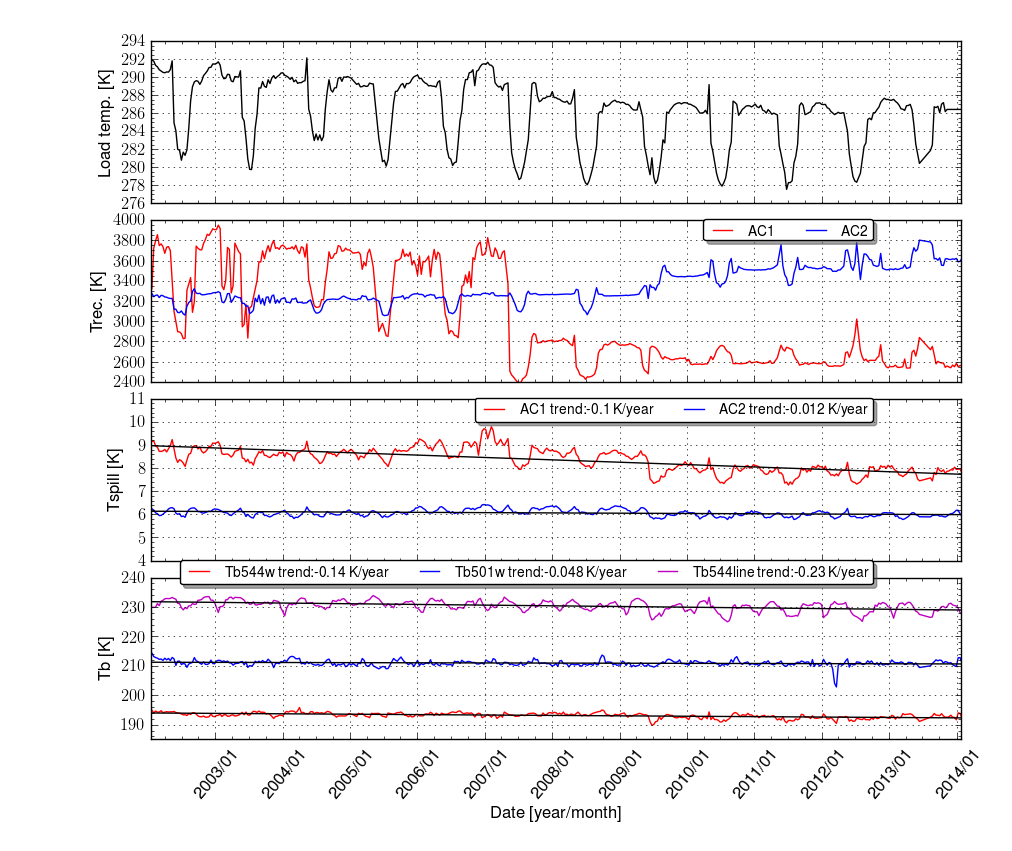
\includegraphics[width=14cm]{tspill_trend3.png}
\caption{Trends in level0/level1b parameters. Upper panel shows the internal
load temperature,
second panel receiver noise temperature, third panel shows \(T_{sp}\) temperature,
and bottom panel shows calibrated brightness temperatures from stratospheric FM1
and FM2 measurements (see text for details) during 2002--2014. Each datapoint
in the figure represents a 10 day average.}
\label{fig:tbtrend}
\end{figure}


Figure~\ref{fig:tbtrend} displays trends in level0/level1b parameters, including brightness 
temperature from stratospheric FM 1 and 2. Tb501w and Tb544w represent the average
Tb within frequency bands around 501.2 and 544.4 GHz, respectively. Tb544line represents Tb around the
strong ozone transition around 544.8 GHz. The figure only contains data from measurements
that correspond to low tangent points (below 9~km) within the tropical region.
A negative trend (measurements being colder with time) can be noted in the figure.
The trend is greater for the 544 GHz band. This trend is not completely understood.

%The internal load temperature is relatively cold during the northern hemisphere summer
%months, since the satellite is then partly in shadow, while the satellite always sees
%the sun otherwise.   


   
\chapter{Comparison of data from different calibration versions}

The current operational \smr\ level2 processing at Chalmers is based on 
Level1B calibration version 7 (L1B-v7) data. 
The L1B-v7 is known to have some issues, and a new calibration version
(L1B-v8) has been developed. The L1B-v8 builds upon the the L1B-v7 algorithm,
but some changes have been applied, with the natural aim to reduce these issues.  

\begin{itemize}

\item L1B-v7 algorithm is orbit based, in the sense that some calibration parameters (\(T_{rec}\)
and \(T_{sp}\)) are common for all scans from a given orbit and frequency mode.
L1B-v8 is scan based, as desribed in Chapter 2.
 
\item L1B-v8 is more strict when it comes to selecting which reference measurements to use.
The movement of an internal mirror can affect the reference measurements when switching
towards the internal load, with a negative impact on final atmospheric
spectra. A more adequate and standardised removal of spectra that are possibly 
affected by the mirror movement is performed in L1B-v8 compared to in L1B-v7. 

\item L1B-v8 also make sures that the instruments settings are the identical
for all spectra that will be calibrated with shared parameters. For most data
this was not issue with L1B-v7, as the instruments settings are most often
only changed when switching observation mode.   


\item L1B-v8 aims for removing ripple seen in calibrated measurements in the
upper part of the scan (see Figure~\ref{fig:ripple}).

\end{itemize}


\begin{figure}
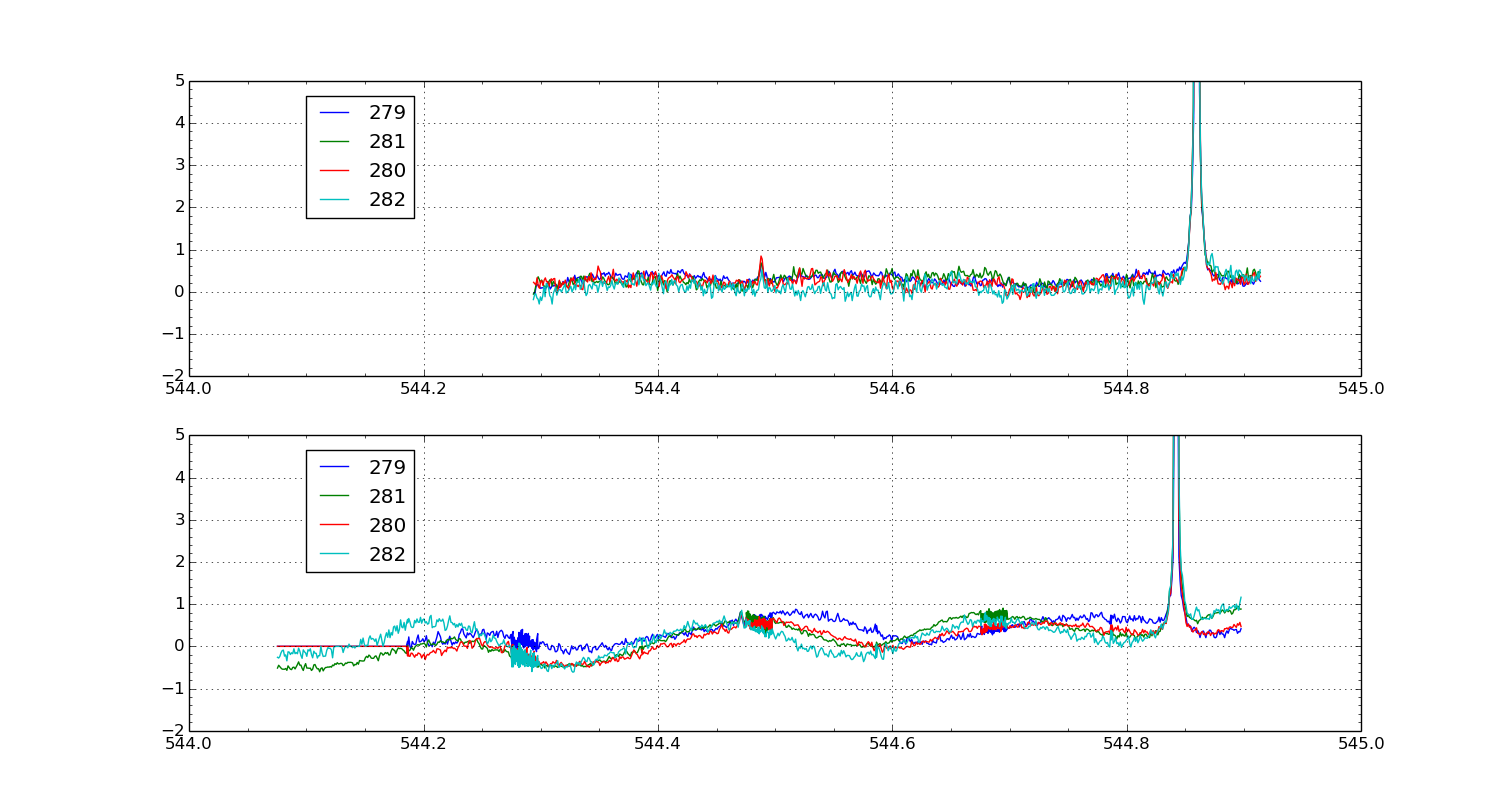
\includegraphics[width=14cm]{ripple_v7and8_FM2_may2009.png}
\caption{Upper panel shows averages of calibrated spectra (verison 8) from measurements
with tangent altitudes above 60\,km for one of the most used frequency modes (FM 2) for May 2009.
The colorcoding/legend corresponds to the ambient temperature or load temperature.
The lower panel shows corresponding data, but for calibration version 7 data.}
%\lcomment{BR}{produce better looking figures} }
\label{fig:ripple}
\end{figure}




%%% Local Variables: 
%%% mode: latex
%%% TeX-master: "L1_ATBD"
%%% End: 
